
\chapter{Measurement of Efficiency of Single Electron Trigger}

\begin{figure}
    \centering
    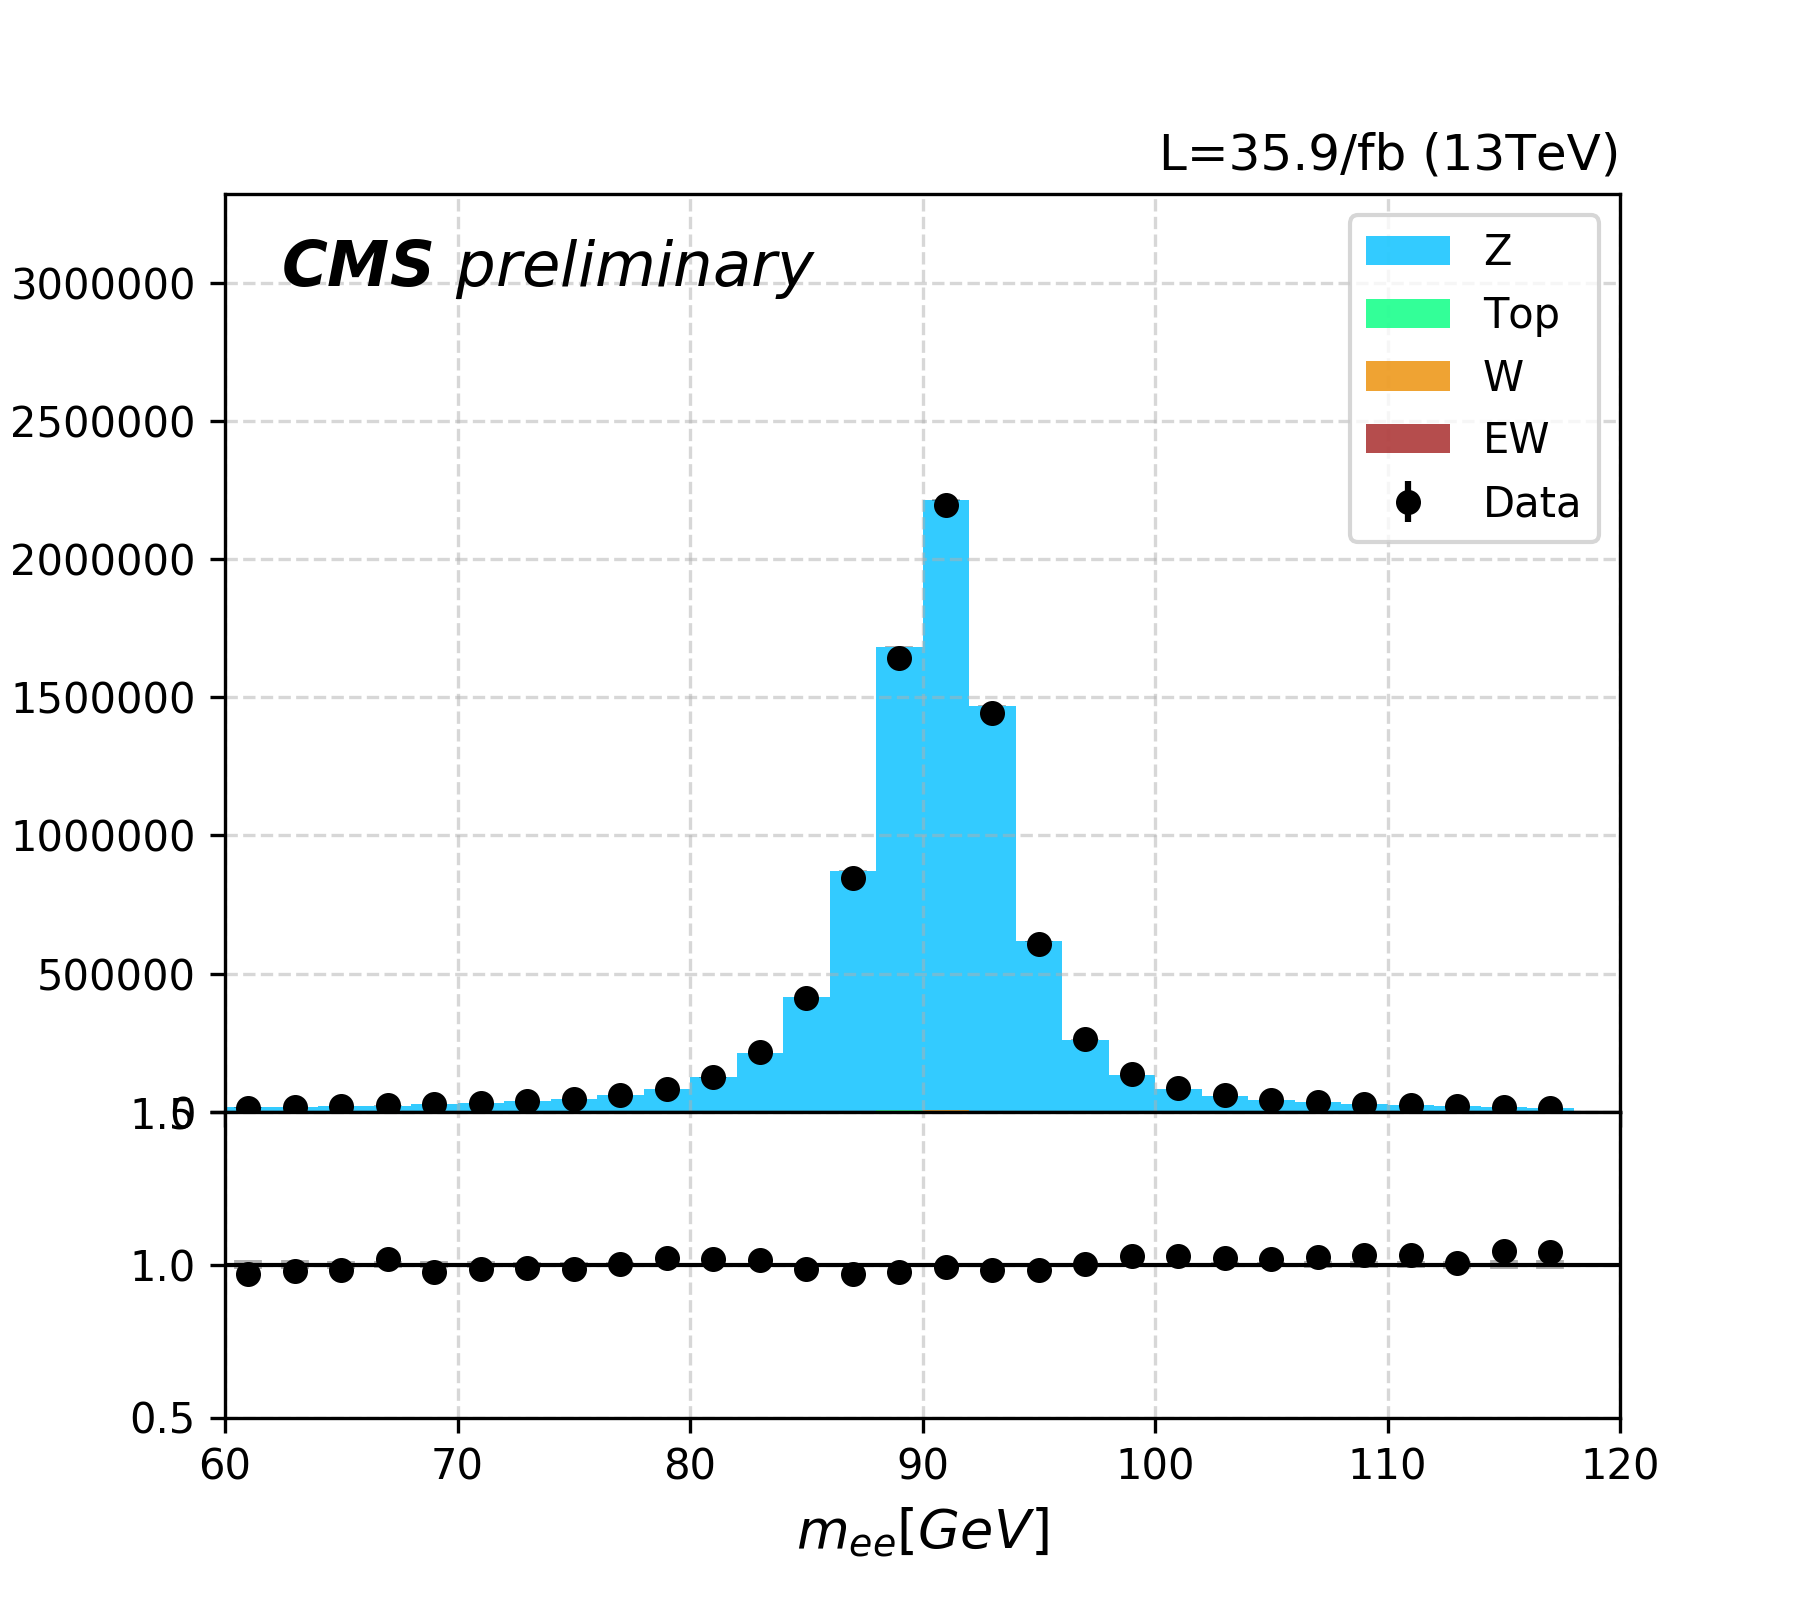
\includegraphics[width=0.6\textwidth]{appendices/ele27TriggerEff/figures/dileptonMass_tag30.png}
    \caption{caption}
    \label{fig:appendix:ele27TriggerSF}
\end{figure}



\begin{figure}
    \centering
    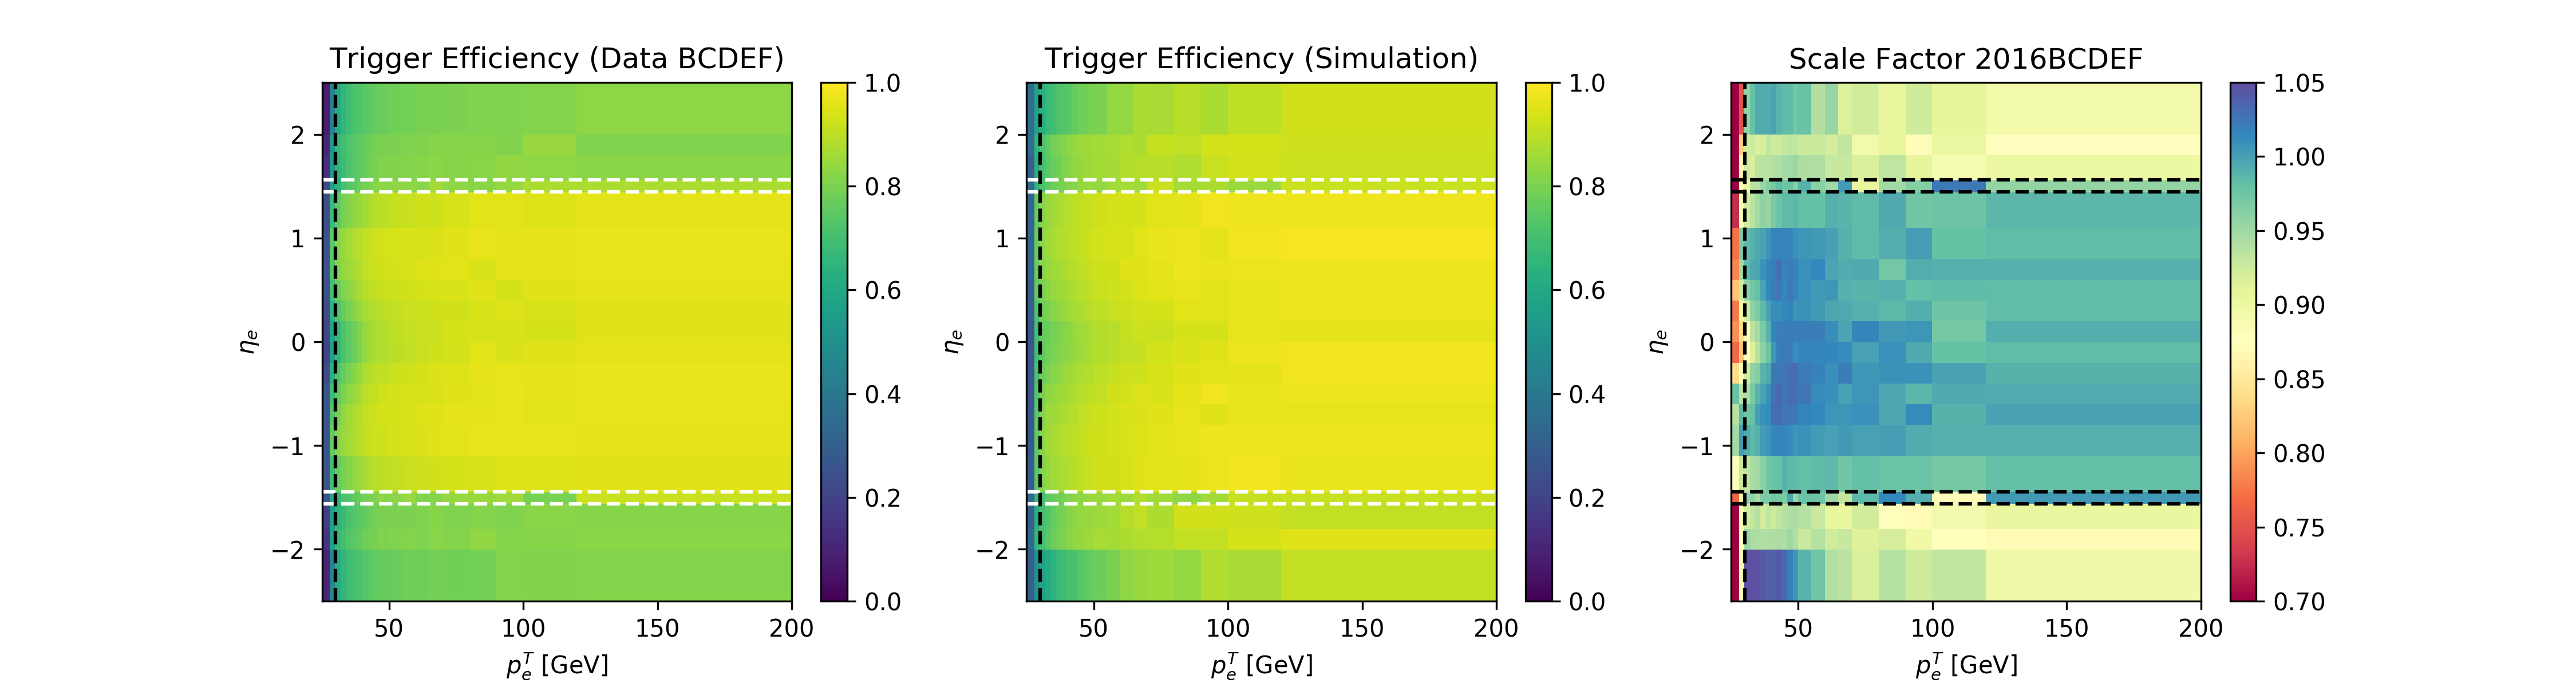
\includegraphics[width=0.99\textwidth]{appendices/ele27TriggerEff/figures/eff2d_BCDEF.png}
    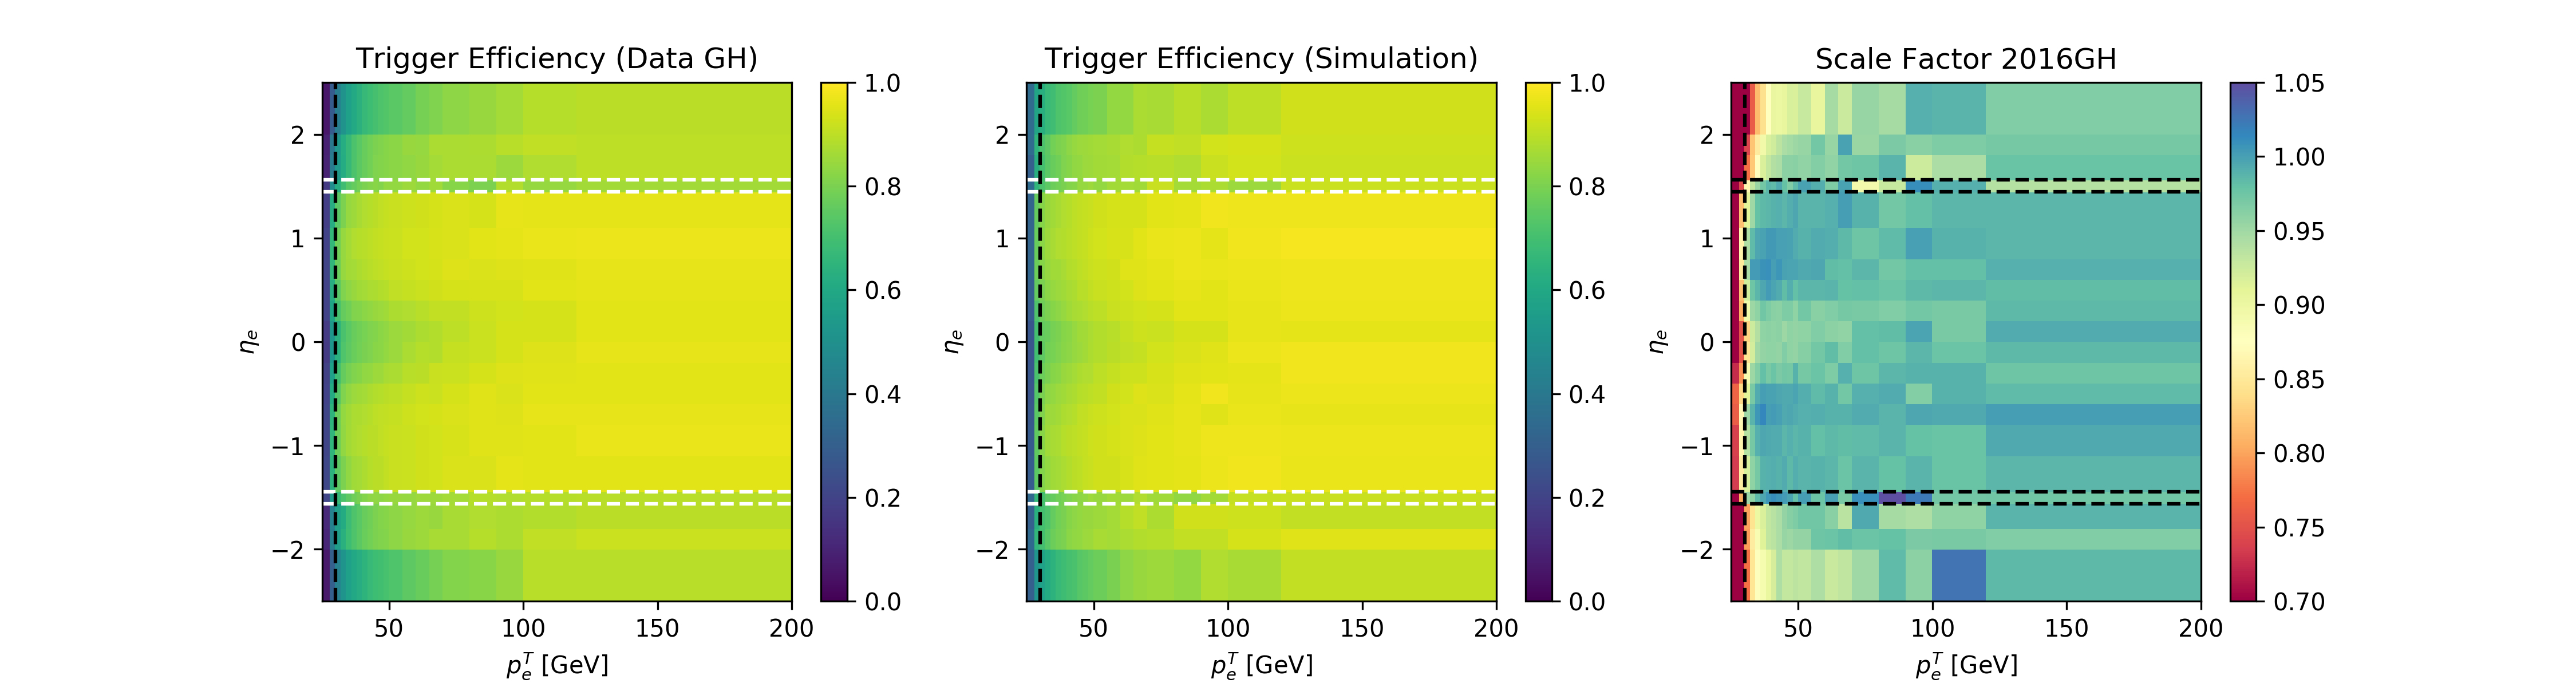
\includegraphics[width=0.99\textwidth]{appendices/ele27TriggerEff/figures/eff2d_GH.png}
    \caption{Reweight $\tau_h$ and $j \to \tau_h$ efficiencies in the dedicated FSR, ISF, MEPS, UE ttbar samples}
    \label{fig:appendix:ele27SF}
\end{figure}


\begin{figure}
    \centering
    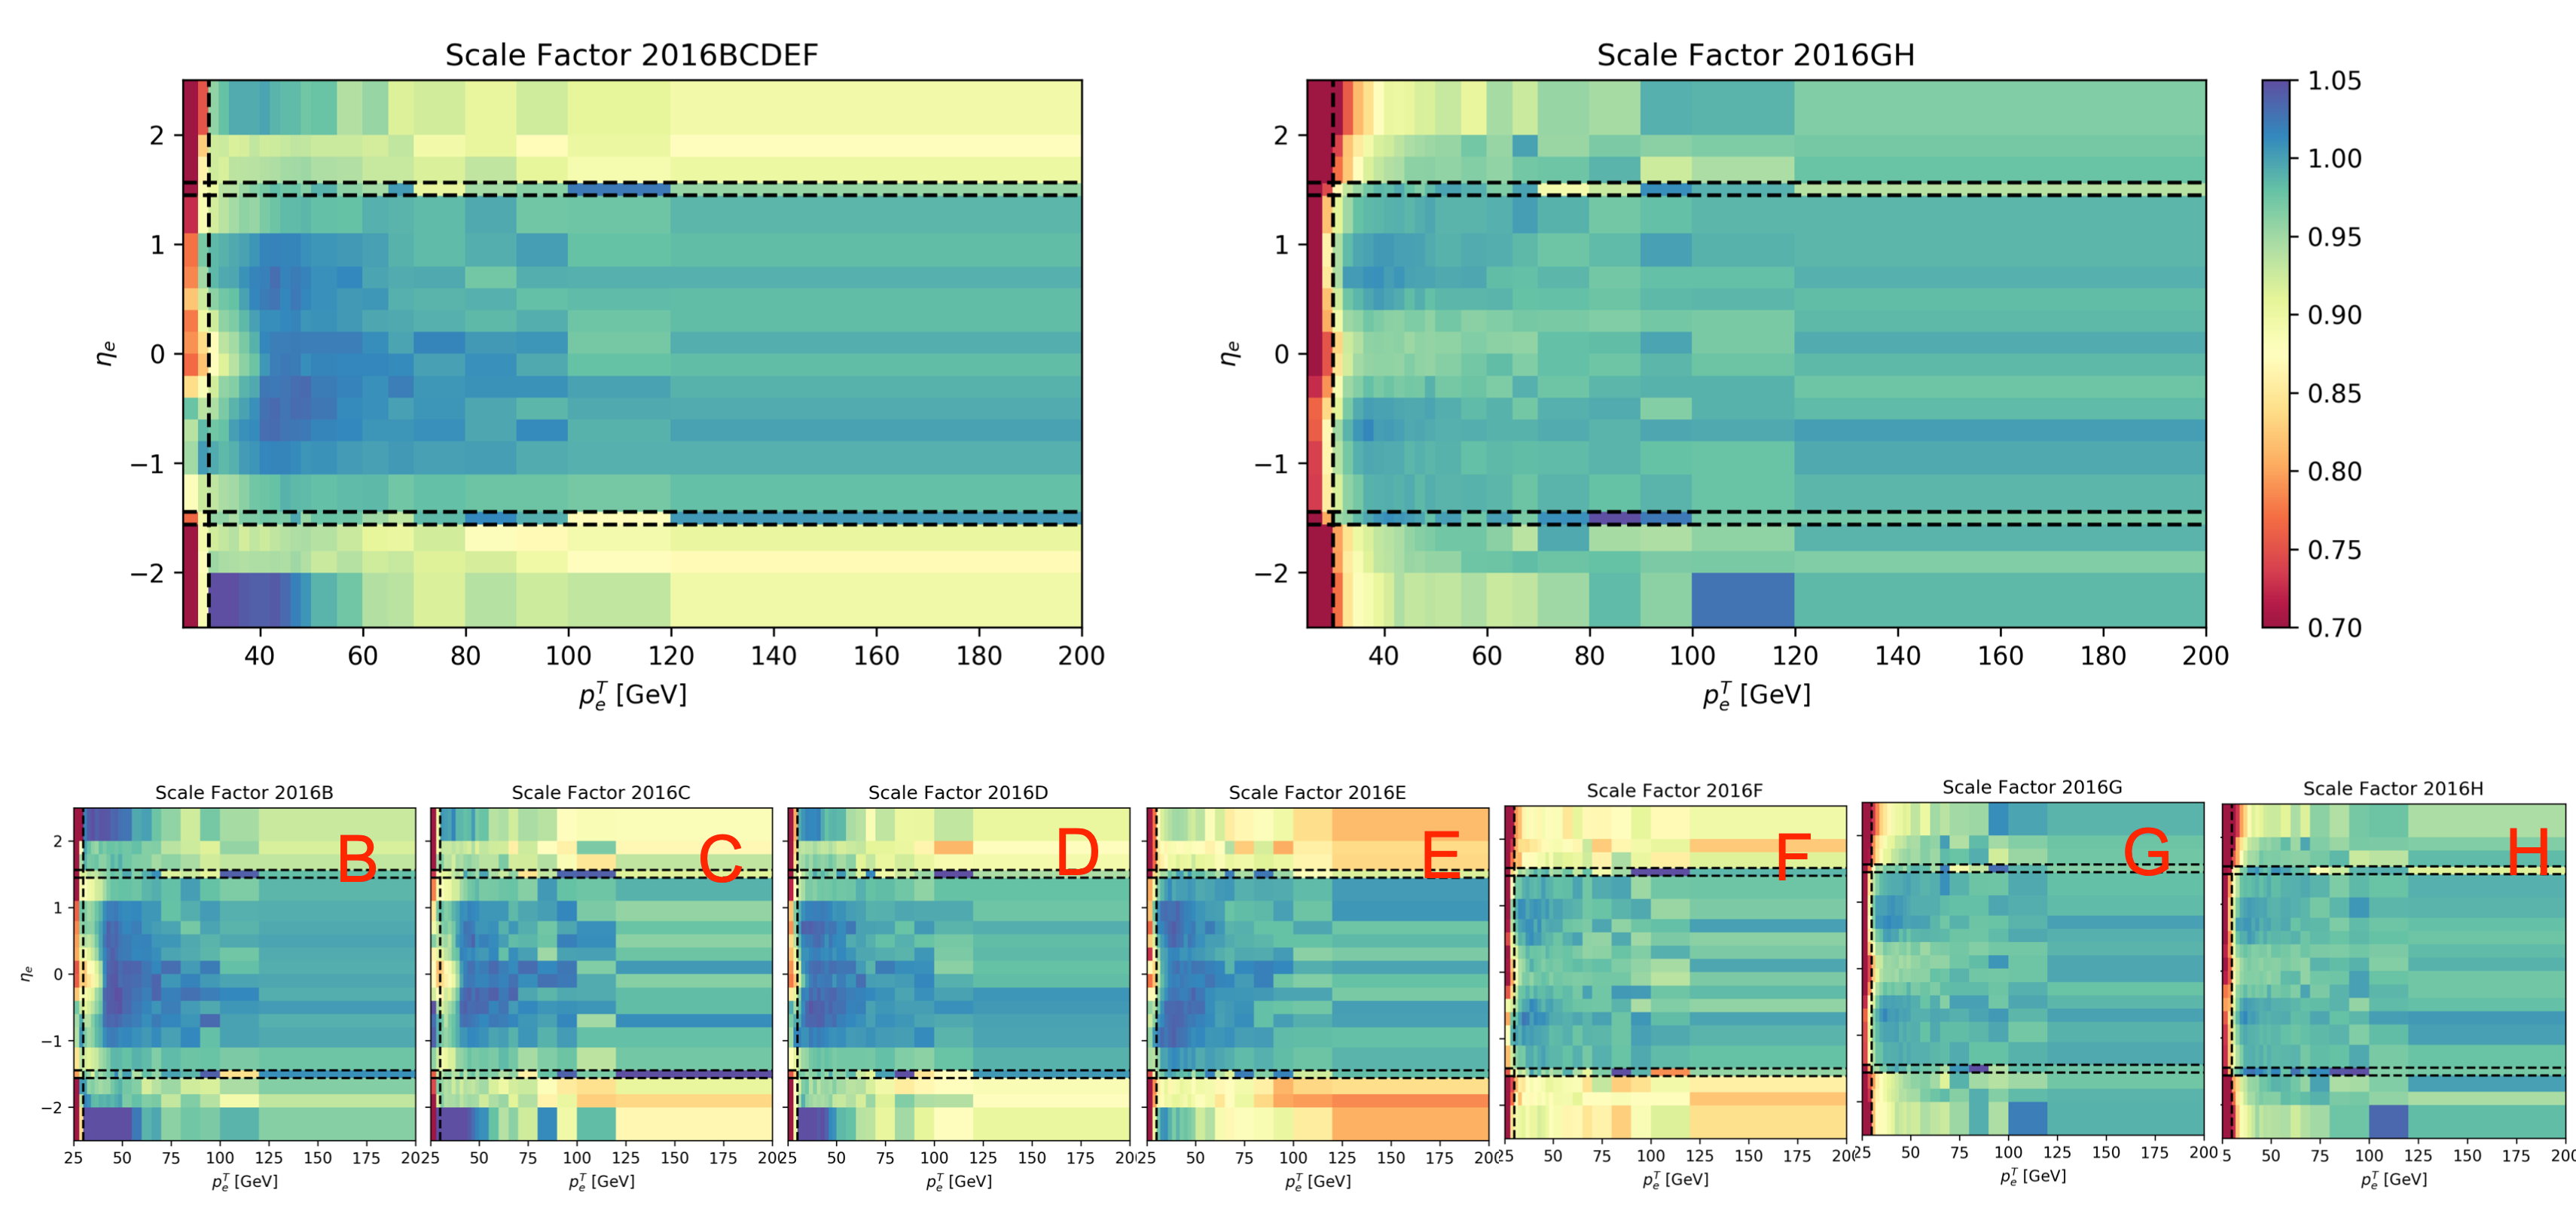
\includegraphics[width=0.99\textwidth]{appendices/ele27TriggerEff/figures/eTrSF_value.png}
    \caption{Reweight $\tau_h$ and $j \to \tau_h$ efficiencies in the dedicated FSR, ISF, MEPS, UE ttbar samples}
    \label{fig:appendix:ele27SF}
\end{figure}





\begin{figure}
    \centering
    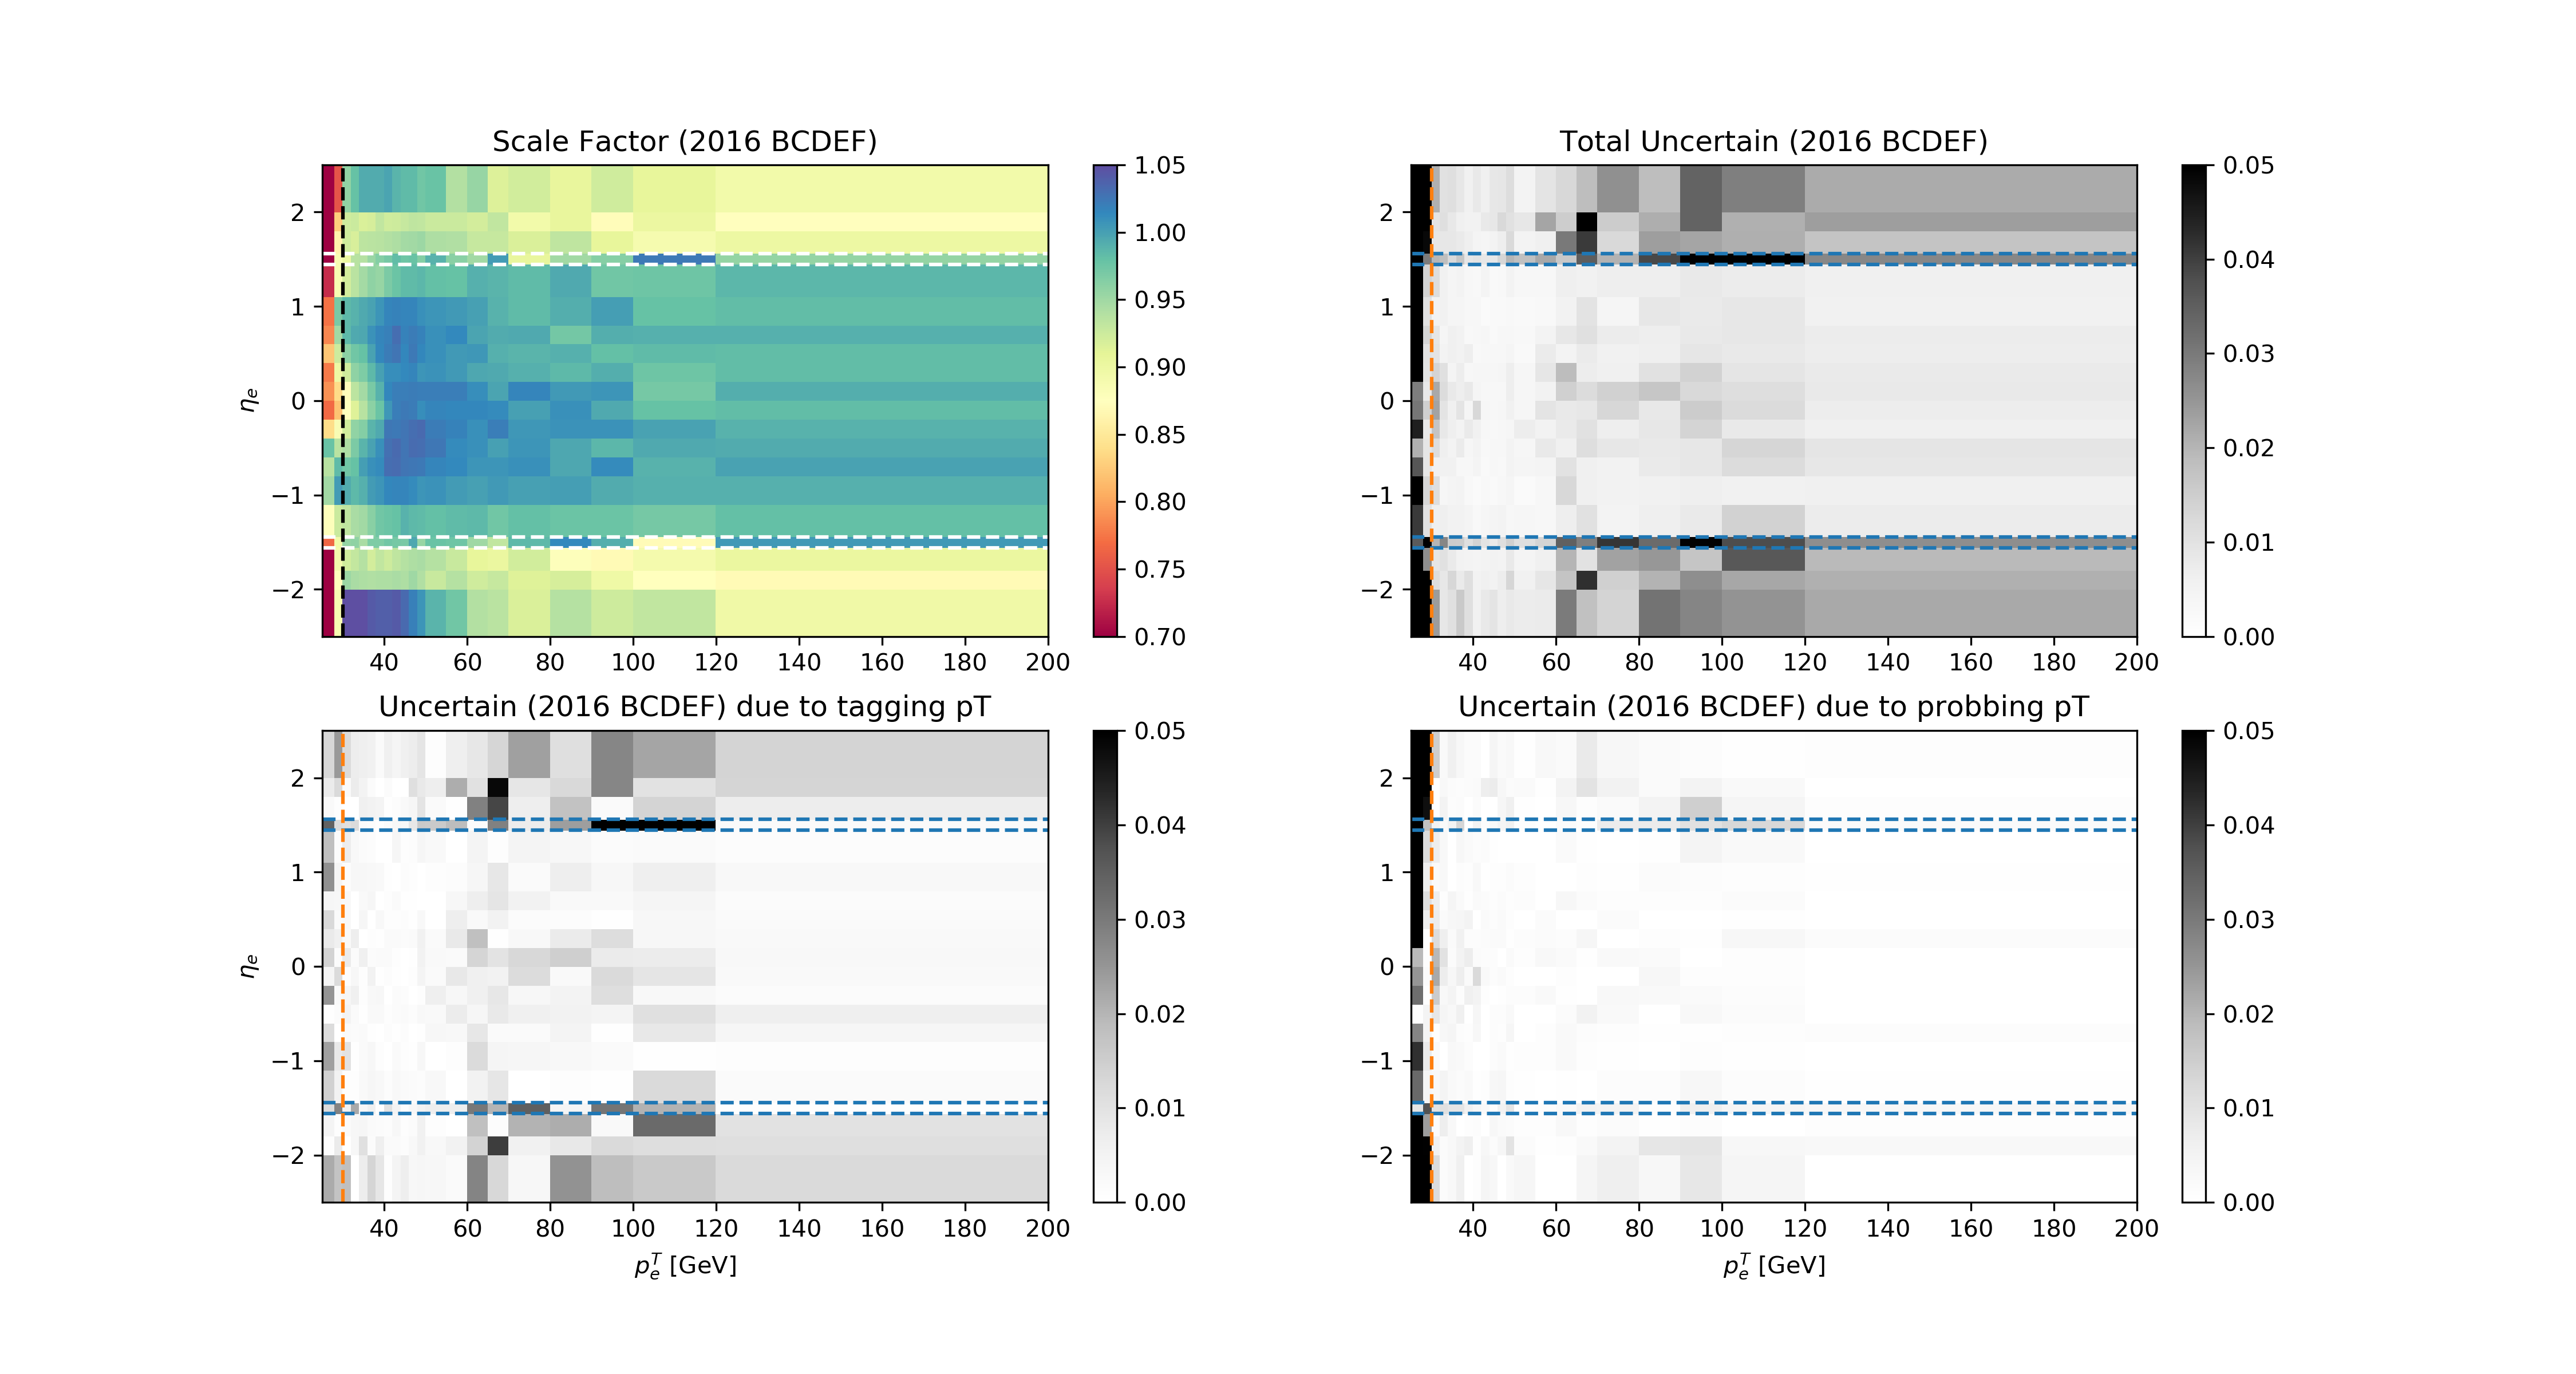
\includegraphics[width=0.99\textwidth]{appendices/ele27TriggerEff/figures/result_BCDEF.png}
    
    \caption{caption}
    \label{fig:appendix:ele27SF}
\end{figure}

\begin{figure}
    \centering
    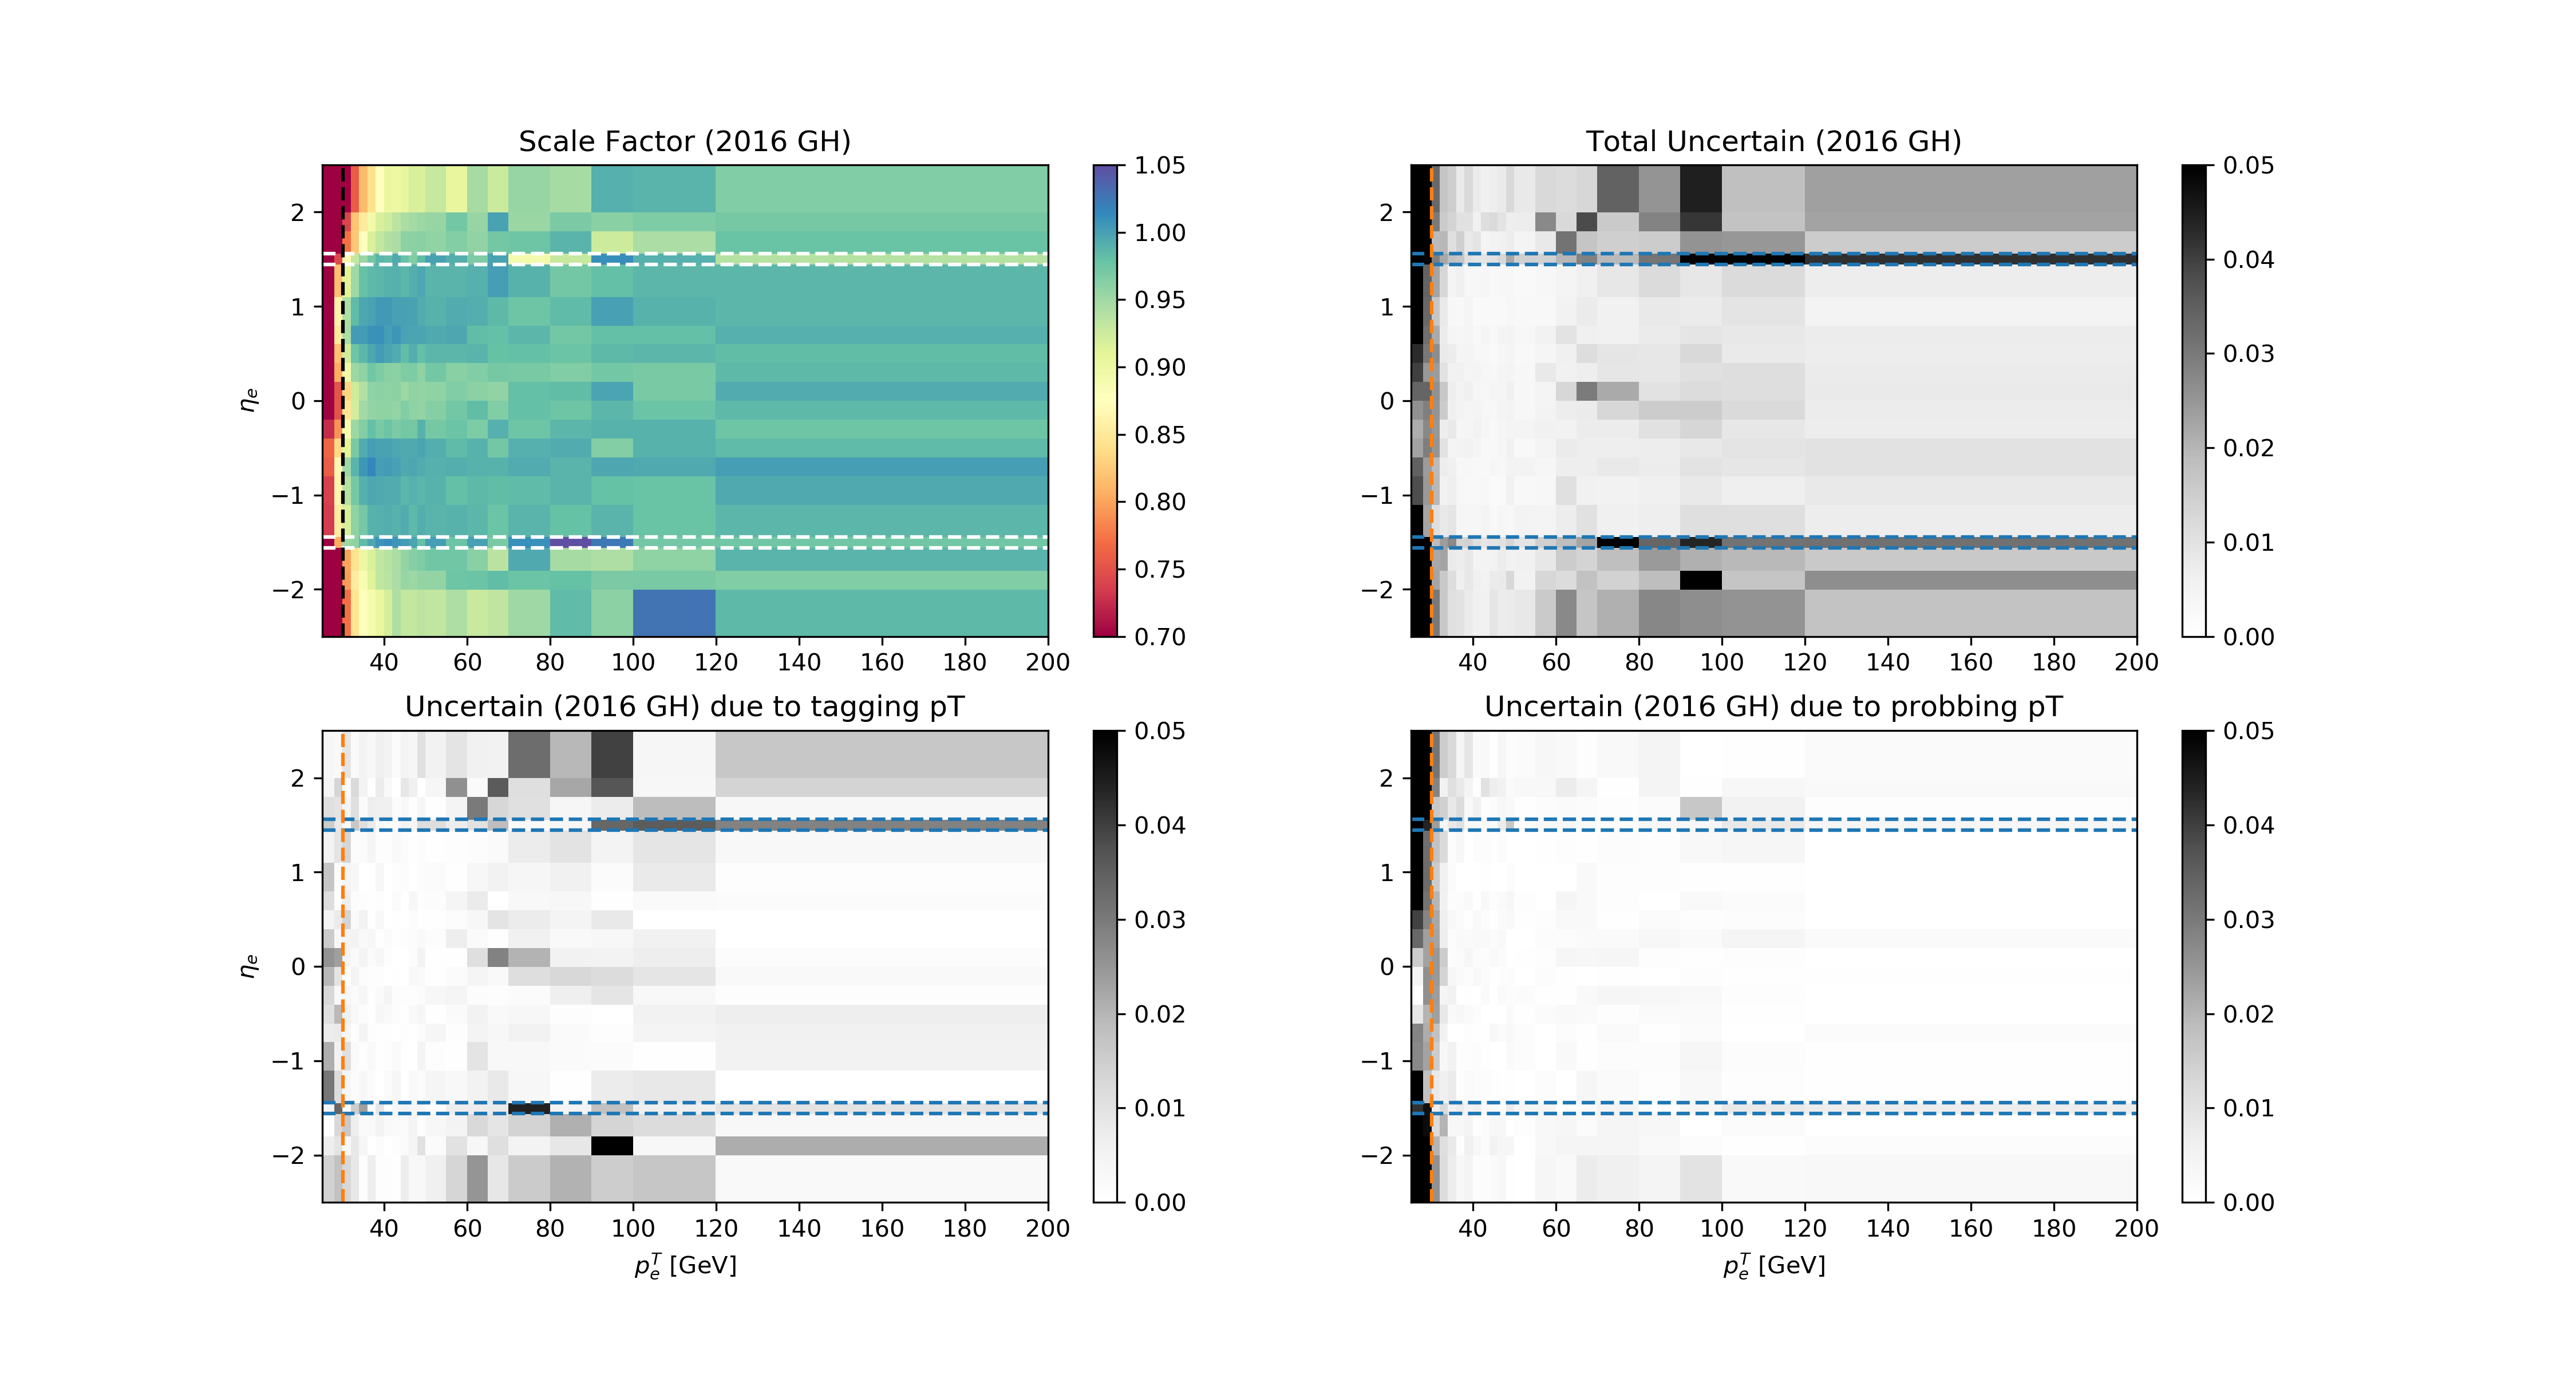
\includegraphics[width=0.99\textwidth]{appendices/ele27TriggerEff/figures/result_GH.png}
    
    \caption{caption}
    \label{fig:appendix:ele27SF}
\end{figure}
